\documentclass[12pt]{article}
\usepackage[utf8]{inputenc}
\usepackage[spanish]{babel}
\usepackage{listings}
\usepackage{xcolor}
\usepackage{graphicx}
\usepackage[colorlinks=true, linkcolor=black, urlcolor=blue]{hyperref}
\usepackage{float}
\usepackage{amsmath}
\usepackage{afterpage}

% Configuración para listings
\definecolor{vscodebg}{RGB}{255, 255, 255}
\definecolor{vscodekeyword}{RGB}{0, 0, 255}
\definecolor{vscodestring}{RGB}{163, 21, 21}
\definecolor{vscodecomment}{RGB}{0, 128, 0}
\definecolor{vscodenumber}{RGB}{9, 134, 88}
\definecolor{vscodeoperator}{RGB}{0, 0, 0}
\definecolor{vscodevariable}{RGB}{0, 16, 128}
\definecolor{vscodetype}{RGB}{38, 127, 153}
\definecolor{vscodelightblue}{RGB}{0, 0, 139}
\definecolor{vscodelinenumber}{RGB}{237, 237, 237}
\definecolor{vscodenumberfg}{RGB}{160, 160, 160}
\definecolor{vscodeborder}{RGB}{240, 240, 240}

\lstset{
    language=Java,
    basicstyle=\ttfamily\footnotesize\color{black},
    backgroundcolor=\color{vscodebg},
    keywordstyle=\color{vscodekeyword},
    commentstyle=\color{vscodecomment},
    stringstyle=\color{vscodestring},
    emphstyle=\color{vscodetype},
    numbers=left,
    numberstyle={\tiny\color{vscodenumberfg}},
    numbersep=8pt,
    breaklines=true,
    frame=single,
    rulecolor=\color{vscodeborder},
    framesep=3pt,
    xleftmargin=0pt,
    xrightmargin=0pt,
    framexleftmargin=8pt,
    framexrightmargin=8pt,
    framextopmargin=2pt,
    framexbottommargin=2pt,
    tabsize=4,
    showstringspaces=false,
    captionpos=b,
    escapeinside={(*@}{@*)},
    emph={String,StringBuilder,System,List,Integer,ArrayList,Override,boolean},
    morekeywords={private,public,class,void,int,final,implements,return,this,new,true,false},
    keywordstyle=\color{vscodekeyword},
    morestring=[b]",
    morecomment=[l]{//},
    morecomment=[s]{/*}{*/},
    numberfirstline=true,
    stepnumber=1,
    firstnumber=1,
    numberblanklines=true,
    literate=
        {ñ}{{\~n}}1
        {Ñ}{{\~N}}1
        {á}{{\\'a}}1
        {é}{{\\'e}}1
        {í}{{\\'i}}1
        {ó}{{\\'o}}1
        {ú}{{\\'u}}1
        {Á}{{\\'A}}1
        {É}{{\\'E}}1
        {Í}{{\\'I}}1
        {Ó}{{\\'O}}1
        {Ú}{{\\'U}}1
        {ü}{{\\\"u}}1
        {¡}{{\\textexclamdown}}1
        {¿}{{\\textquestiondown}}1
        {>>>}{{\color{vscodeoperator}>>>}}3
        {<=}{{\color{vscodeoperator}<=}}2
        {>=}{{\color{vscodeoperator}>=}}2
        {==}{{\color{vscodeoperator}==}}2
        {=}{{\color{vscodeoperator}=}}1
        {+}{{\color{vscodeoperator}+}}1
        {-}{{\color{vscodeoperator}-}}1
        {*}{{\color{vscodeoperator}*}}1
        {/}{{\color{vscodeoperator}/}}1
        {!}{{\color{vscodeoperator}!}}1
        {[}{{\color{vscodeoperator}[}}1
        {]}{{\color{vscodeoperator}]}}1
        {<}{{\color{vscodeoperator}<}}1
        {>}{{\color{vscodeoperator}>}}1
        {(}{{\color{vscodeoperator}(}}1
        {)}{{\color{vscodeoperator})}}1
        {.}{{\color{vscodeoperator}.}}1
        {,}{{\color{vscodeoperator},}}1
        {;}{{\color{vscodeoperator};}}1
        {:}{{\color{vscodeoperator}:}}1
        {&&}{{\color{vscodeoperator}&&}}2
        {||}{{\color{vscodeoperator}||}}2
        {!=}{{\color{vscodeoperator}!=}}2
        {&}{{\color{vscodeoperator}\&}}1,
    numberbychapter=false,
    resetmargins=true
}

\title{Taller 7: Optimización de Matriz de Costos con Backtracking Paralelo con Threads en Java}
\author{
  Cristian Bravo \\
  Bruno Bastidas \\
  Silvio Villagra \\
  Daniella Lecanda \\[2ex]
  \textbf{Grupo investigativo Los Catalizadores}
}
\date{07/05/2025}

\begin{document}

\maketitle
\clearpage

\section*{Introducción}

En el presente taller, abordamos el desafío de paralelizar un algoritmo de backtracking para encontrar el camino más corto en un grafo, utilizando threads en Java. El backtracking es una técnica de búsqueda exhaustiva que explora todas las posibles soluciones mediante recursión, retrocediendo cuando una solución parcial no puede extenderse a una solución válida. Aunque efectivo, este enfoque puede volverse computacionalmente costoso para problemas de gran escala, lo que hace necesaria la implementación de estrategias de paralelización para mejorar su rendimiento.

Nuestra implementación se desarrolló en Java, aprovechando su robustez y facilidad para manejar concurrencia mediante threads. Java permite la creación y gestión directa de hilos, lo que posibilita la exploración de múltiples ramas del árbol de búsqueda de manera simultánea.

Para lograr una solución eficiente y escalable, aplicamos las siguientes estrategias basadas en el análisis del código proporcionado:
\begin{itemize}
    \item \textbf{Paralelización con threads Java}: Dividimos el espacio de búsqueda, específicamente las exploraciones iniciales desde el nodo de partida, asignando conjuntos de movimientos iniciales a diferentes threads. Cada thread explora una porción del árbol de búsqueda de forma independiente. Esto se observa en la clase `ParallelGraphSolver`.
    \item \textbf{Uso de estructuras concurrentes}: Empleamos estructuras de datos seguras para hilos como `AtomicInteger` para gestionar el mejor costo encontrado de manera atómica y `ConcurrentLinkedQueue` para almacenar los mejores caminos encontrados por los diferentes hilos, evitando condiciones de carrera y garantizando la consistencia de los resultados.
    \item \textbf{Gestión manual de threads}: La creación, inicio (`thread.start()`) y espera (`thread.join()`) de threads se gestiona directamente en el código, lo que proporciona un control granular sobre el ciclo de vida de los hilos paralelos.
    \item \textbf{Evaluación del rendimiento}: Comparamos el rendimiento del algoritmo secuencial frente al paralelizado, midiendo los tiempos de ejecución para diferentes tamaños de matrices y registrando estos tiempos utilizando una clase `TimeLogger`. Este análisis nos permite determinar en qué casos la paralelización justifica su implementación.
\end{itemize}

El objetivo final de este estudio es demostrar empíricamente cómo la paralelización del algoritmo de backtracking en Java puede mejorar su rendimiento, especialmente en problemas con un gran espacio de búsqueda. A través de este taller, exploramos las ventajas y limitaciones de la paralelización con threads, proporcionando una comprensión más profunda de su aplicabilidad en algoritmos de optimización de caminos.

\section*{Componentes Clave del Sistema}
El sistema se compone de las siguientes clases principales:
\begin{itemize}
    \item \textbf{GraphBacktrackingProblem}: Modela el problema del camino más corto en un grafo usando una matriz de adyacencia. Gestiona el estado del recorrido, el costo acumulado y los movimientos posibles.
    \item \textbf{SequentialGraphSolver}: Implementa el algoritmo de backtracking de forma secuencial, explorando todas las rutas posibles desde el nodo inicial al final y actualizando el mejor camino encontrado.
    \item \textbf{ParallelGraphSolver}: Divide la exploración inicial entre varios hilos (threads), permitiendo que cada uno explore diferentes ramas del árbol de búsqueda en paralelo. Utiliza estructuras concurrentes como \texttt{AtomicInteger} y \texttt{ConcurrentLinkedQueue} para evitar condiciones de carrera y asegurar la consistencia de los resultados.
    \item \textbf{MatrixUtils}: Genera matrices aleatorias, orquesta la ejecución de ambos algoritmos y formatea los resultados.
    \item \textbf{TimeLogger}: Registra los tiempos de ejecución y genera un resumen final en archivos de texto para facilitar el análisis posterior.
    \item \textbf{Main}: Es el punto de entrada del programa, configura los parámetros de la simulación y coordina la ejecución de los experimentos.
\end{itemize}

\section*{Principales Componentes del Sistema}

El sistema implementado consta de varias clases Java clave que interactúan para resolver el problema del camino más corto mediante backtracking, tanto de forma secuencial como paralela.

\subsection*{Definición del Problema (`GraphBacktrackingProblem.java`)}
La clase `GraphBacktrackingProblem` encapsula la lógica y el estado del problema de encontrar el camino más corto en un grafo representado por una matriz de adyacencia.

\begin{lstlisting}[caption={Fragmento de `GraphBacktrackingProblem.java`}, morekeywords={Override}]
package cl.unab.fundamentos.app;

import cl.unab.fundamentos.interfaces.BacktrackingProblem;
import java.util.*;

public class GraphBacktrackingProblem implements BacktrackingProblem {
    private final int[][] matrix;
    private final int n;
    private final int start;
    private final int end;
    private List<Integer> bestPath;
    private int bestCost;
    private List<Integer> currentPath;

    public GraphBacktrackingProblem(int[][] matrix, int start, int end) {
        this.matrix = matrix;
        this.n = matrix.length;
        this.start = start;
        this.end = end;
        this.bestPath = new ArrayList<>();
        this.bestCost = Integer.MAX_VALUE;
        this.currentPath = new ArrayList<>();
    }

    @Override
    public boolean isSolution() {
        return !currentPath.isEmpty() && currentPath.get(currentPath.size() - 1) == end;
    }

    @Override
    public void applyMove(int move) {
        if (!currentPath.isEmpty()) {
            currentCost += matrix[currentPath.get(currentPath.size() - 1)][move];
        }
        currentPath.add(move);
        visited[move] = true;
    }

    @Override
    public void undoMove(int move) {
        visited[move] = false;
        currentPath.remove(currentPath.size() - 1);
    }

    @Override
    public List<Integer> getPossibleMoves() {
        List<Integer> moves = new ArrayList<>();
        int last = currentPath.isEmpty() ? start : currentPath.get(currentPath.size() - 1);
        for (int i = 0; i < n; i++) {
            if (!visited[i] && matrix[last][i] != 0 && matrix[last][i] != INF) {
                moves.add(i);
            }
        }
        return moves;
    }
}
\end{lstlisting}
Esta clase maneja el estado actual del camino, el costo, y determina los movimientos posibles, además de verificar si se ha encontrado una solución.

\subsection*{Utilidades de Matriz y Ejecución (`MatrixUtils.java`)}
La clase `MatrixUtils` se encarga de generar las matrices de costos y de orquestar la ejecución de las versiones secuencial y paralela del algoritmo.

\begin{lstlisting}[caption={Fragmento de `MatrixUtils.java`}, morekeywords={Random}]
package cl.unab.fundamentos.utils;

public class MatrixUtils {
    public static final int INF = 9999;

    public static int[][] generarMatriz(int n, Random rand) {
        int[][] matrix = new int[n][n];
        for (int i = 0; i < n; i++) {
            for (int j = 0; j < n; j++) {
                if (i == j) {
                    matrix[i][j] = 0;
                } else {
                    if (rand.nextDouble() < 0.05) { // Probabilidad de INF
                        matrix[i][j] = INF;
                    } else {
                        matrix[i][j] = 1 + rand.nextInt(10); // Costos entre 1 y 10
                    }
                }
            }
        }
        return matrix;
    }

    public static ExecutionResult ejecutarProblema(int n, int numThreads) {
        Random rand = new Random();
        int[][] matrix = generarMatriz(n, rand);

        // Secuencial
        GraphBacktrackingProblem seqProblem = new GraphBacktrackingProblem(matrix, start, end);
        long startSeq = System.nanoTime();
        SequentialGraphSolver seqSolver = new SequentialGraphSolver(seqProblem);
        seqSolver.solve();
        long endSeq = System.nanoTime();
        double tiempoSeq = (endSeq - startSeq) / 1000.0; // Microsegundos

        // Paralelo
        GraphBacktrackingProblem parProblem = new GraphBacktrackingProblem(matrix, start, end);
        long startPar = System.nanoTime();
        ParallelGraphSolver parSolver = new ParallelGraphSolver(parProblem, numThreads);
        parSolver.solve();
        long endPar = System.nanoTime();
        double tiempoPar = (endPar - startPar) / 1000.0; // Microsegundos
        
        TimeLogger.logExecutionTime(n, tiempoSeq, tiempoPar, numThreads);
        return new ExecutionResult(output.toString(), tiempoSeq, tiempoPar);
    }
}
\end{lstlisting}

\subsection*{Registro de Tiempos (`TimeLogger.java`)}
`TimeLogger` es una utilidad para registrar los tiempos de ejecución y un resumen final en archivos de texto, permitiendo el análisis posterior del rendimiento.
\begin{lstlisting}[caption={Fragmento de `TimeLogger.java`}, morekeywords={FileWriter, IOException, LocalDateTime, DateTimeFormatter}]
package cl.unab.fundamentos.utils;

public class TimeLogger {
    private static final String LOG_DIR = "taller-7";

    public static void logExecutionTime(int matrixSize, double seqTime, double parTime, int numThreads) {
        try (FileWriter writer = new FileWriter(LOG_FILE, true)) {
            StringBuilder sb = new StringBuilder();
            sb.append("Matriz ").append(matrixSize).append("x").append(matrixSize).append(":\n");
            sb.append("Tiempo secuencial: ").append(String.format("%.2f", seqTime)).append(" microsegundos\n");
            sb.append("Tiempo paralelo: ").append(String.format("%.2f", parTime)).append(" microsegundos\n");
            if (parTime > 0) {
                sb.append("Speedup: ").append(String.format("%.4f", seqTime/parTime)).append("\n");
            }
            writer.write(sb.toString());
        } catch (IOException e) {
            System.err.println("Error al escribir en el archivo de tiempos: " + e.getMessage());
        }
    }
}
\end{lstlisting}

\section*{Algoritmo Secuencial (`SequentialGraphSolver.java`)}
La clase `SequentialGraphSolver` implementa el algoritmo de backtracking de manera secuencial para encontrar el camino de menor costo.

\begin{lstlisting}[caption={Algoritmo de Backtracking Secuencial en Java (`SequentialGraphSolver.java`)}]
package cl.unab.fundamentos.app;

public class SequentialGraphSolver {
    private final GraphBacktrackingProblem problem;

    public SequentialGraphSolver(GraphBacktrackingProblem problem) {
        this.problem = problem;
    }

    public void solve() {
        boolean[] visited = new boolean[problem.getN()];
        visited[problem.getStart()] = true; // Marcar el nodo inicial como visitado
        backtrack(problem.getStart(), visited, 0); // Costo es 0 para alcanzar el nodo inicial
    }

    private void backtrack(int node, boolean[] visited, int currentCost) {
        // Si el nodo actual es el destino
        if (node == problem.getEnd()) {
            if (currentCost < problem.getBestCost()) {
                problem.setBestCost(currentCost);
                problem.setBestPath(problem.getCurrentPath()); // Guardar camino actual como el mejor
            }
            return; // Retroceder
        }

        // Explorar vecinos
        for (int next = 0; next < problem.getN(); next++) {
            // Si 'next' es un vecino válido, no visitado con una arista no-INF
            if (!visited[next] && problem.getMatrix()[node][next] != 0 && 
                problem.getMatrix()[node][next] != GraphBacktrackingProblem.INF) {
                
                visited[next] = true;       // Marcar como visitado
                problem.addToPath(next);    // Agregar al camino actual
                
                backtrack(next, visited, currentCost + problem.getMatrix()[node][next]);
                
                problem.removeFromPath();   // Remover del camino actual
                visited[next] = false;      // Desmarcar como visitado
            }
        }
    }
}
\end{lstlisting}
El método `solve` inicia el proceso, y `backtrack` explora recursivamente los caminos posibles, actualizando el mejor camino encontrado.

\section*{Implementación Paralela con Threads (`ParallelGraphSolver.java`)}
La clase `ParallelGraphSolver` paraleliza el algoritmo de backtracking utilizando threads. Divide la exploración de los movimientos iniciales desde el nodo de partida entre varios threads.

\begin{lstlisting}[caption={Implementación Paralela con Threads en Java (`ParallelGraphSolver.java`)}]
package cl.unab.fundamentos.app;

import java.util.List;
import java.util.ArrayList;
import java.util.concurrent.atomic.AtomicInteger;
import java.util.concurrent.ConcurrentLinkedQueue;

public class ParallelGraphSolver {
    private final GraphBacktrackingProblem problem;
    private final int numThreads;
    private final AtomicInteger bestCost; // Mejor costo compartido
    private final ConcurrentLinkedQueue<List<Integer>> bestPaths; // Lista compartida de mejores caminos

    public ParallelGraphSolver(GraphBacktrackingProblem problem, int numThreads) {
        this.problem = problem;
        this.numThreads = Math.min(numThreads, problem.getPossibleMoves().size() > 0 ? problem.getPossibleMoves().size() : 1);
        this.bestCost = new AtomicInteger(Integer.MAX_VALUE);
        this.bestPaths = new ConcurrentLinkedQueue<>();
        if (this.problem != null) {
             this.problem.setBestCost(Integer.MAX_VALUE);
        }
    }

    public void solve() {
        List<Thread> threads = new ArrayList<>();
        List<Integer> initialMoves = problem.getPossibleMoves(); 

        if (initialMoves.isEmpty() && problem.getStart() == problem.getEnd()) {
            // Manejar caso donde inicio y fin son iguales
            problem.setBestCost(0);
            problem.setBestPath(new ArrayList<>(List.of(problem.getStart())));
            bestCost.set(0);
            bestPaths.offer(new ArrayList<>(List.of(problem.getStart())));
            return;
        }
        
        int effectiveNumThreads = Math.min(this.numThreads, initialMoves.size());
        if (effectiveNumThreads == 0 && !initialMoves.isEmpty()) effectiveNumThreads = 1;
        if (initialMoves.isEmpty()) effectiveNumThreads = 0;

        int movesPerThread = (initialMoves.size() + effectiveNumThreads - 1) / effectiveNumThreads;

        for (int i = 0; i < effectiveNumThreads; i++) {
            final int threadId = i;
            GraphBacktrackingProblem threadProblemInstance = new GraphBacktrackingProblem(this.problem);
            
            threadProblemInstance.addToPath(threadProblemInstance.getStart());
            boolean[] initialVisited = new boolean[threadProblemInstance.getN()];
            initialVisited[threadProblemInstance.getStart()] = true;

            Thread thread = new Thread(() -> {
                int startMoveIndex = threadId * movesPerThread;
                int endMoveIndex = Math.min((threadId + 1) * movesPerThread, initialMoves.size());

                for (int moveIdx = startMoveIndex; moveIdx < endMoveIndex; moveIdx++) {
                    int move = initialMoves.get(moveIdx);
                    
                    boolean[] visitedCurrentMove = Arrays.copyOf(initialVisited, initialVisited.length);
                    
                    if (!visitedCurrentMove[move]) {
                        visitedCurrentMove[move] = true;
                        threadProblemInstance.addToPath(move);
                        
                        int costToReachMove = threadProblemInstance.getMatrix()[threadProblemInstance.getStart()][move];
                        
                        backtrack(threadProblemInstance, move, visitedCurrentMove, costToReachMove);
                        
                        threadProblemInstance.removeFromPath();
                    }
                }
            });
            threads.add(thread);
            thread.start();
        }

        for (Thread thread : threads) {
            try {
                thread.join();
            } catch (InterruptedException e) {
                Thread.currentThread().interrupt();
                e.printStackTrace();
            }
        }

        if (bestCost.get() < this.problem.getBestCost()) {
            this.problem.setBestCost(bestCost.get());
            if (!bestPaths.isEmpty()) {
                 this.problem.setBestPath(new ArrayList<>(bestPaths.peek()));
            }
        }
    }

    private void backtrack(GraphBacktrackingProblem currentProblem, int currentNode, 
                           boolean[] visited, int accumulatedCost) {
        if (accumulatedCost >= bestCost.get()) {
            return; // Poda: si el costo actual es peor que el mejor global, detener
        }

        if (currentNode == currentProblem.getEnd()) {
            int oldGlobalBestCost;
            do {
                oldGlobalBestCost = bestCost.get();
                if (accumulatedCost < oldGlobalBestCost) {
                    if (bestCost.compareAndSet(oldGlobalBestCost, accumulatedCost)) {
                        bestPaths.clear();
                        bestPaths.offer(new ArrayList<>(currentProblem.getCurrentPath()));
                        break;
                    }
                } else if (accumulatedCost == oldGlobalBestCost) {
                     bestPaths.offer(new ArrayList<>(currentProblem.getCurrentPath()));
                     break;
                } else {
                    break;
                }
            } while (true);
            return;
        }

        // Explorar vecinos
        for (int nextNode = 0; nextNode < currentProblem.getN(); nextNode++) {
            int edgeCost = currentProblem.getMatrix()[currentNode][nextNode];
            if (!visited[nextNode] && edgeCost != 0 && edgeCost != GraphBacktrackingProblem.INF) {
                if (accumulatedCost + edgeCost < bestCost.get()) {
                    visited[nextNode] = true;
                    currentProblem.addToPath(nextNode);
                    
                    backtrack(currentProblem, nextNode, visited, accumulatedCost + edgeCost);
                    
                    currentProblem.removeFromPath();
                    visited[nextNode] = false;
                }
            }
        }
    }
}
\end{lstlisting}
Utiliza `AtomicInteger` para el `bestCost` global y `ConcurrentLinkedQueue` para `bestPaths` para garantizar la seguridad en el acceso concurrente.

\section*{Orquestación Principal (`Main.java`)}
La clase `Main` es el punto de entrada de la aplicación. Configura los parámetros de la simulación (tamaño mínimo y máximo de la matriz, número de threads) e itera a través de los diferentes tamaños de matriz, ejecutando las versiones secuencial y paralela del algoritmo y registrando los resultados.

\begin{lstlisting}[
    caption={Clase Principal (`Main.java`)},
    language=Java,
    numbers=left,
    numberstyle=\tiny\color{gray},
    numbersep=5pt,
    frame=single,
    framesep=3pt,
    rulecolor=\color{gray!30},
    backgroundcolor=\color{gray!5},
    basicstyle=\ttfamily\small,
    keywordstyle=\color{blue}\bfseries,
    commentstyle=\color{green!50!black}\itshape,
    stringstyle=\color{orange},
    showstringspaces=false,
    breaklines=true,
    xleftmargin=20pt,
    xrightmargin=10pt
]
package cl.unab.fundamentos;

import cl.unab.fundamentos.utils.MatrixUtils;
import cl.unab.fundamentos.utils.TimeLogger;

public class Main {
    private static final int MAX_SIZE = 14;    // Tamaño máximo de matriz NxN
    private static final int MIN_SIZE = 2;     // Tamaño mínimo de matriz NxN
    private static final int NUM_THREADS = 16; // Número de hilos para ejecución paralela

    public static void main(String[] args) {
        StringBuilder output = new StringBuilder();
        System.out.print(output.toString());

        double totalSeqTime = 0;
        double totalParTime = 0;

        // Iterar sobre diferentes tamaños de matriz
        for (int n = MIN_SIZE; n <= MAX_SIZE; n++) {
            MatrixUtils.ExecutionResult result = 
                MatrixUtils.ejecutarProblema(n, NUM_THREADS);
            System.out.print(result.output);
            
            totalSeqTime += result.tiempoSecuencial;
            totalParTime += result.tiempoParalelo;
        }

        // Generar resumen final de todas las ejecuciones
        TimeLogger.logFinalSummary(MAX_SIZE, totalSeqTime, totalParTime);
    }
}
\end{lstlisting}

\section*{Compilación y Ejecución}

Para compilar y ejecutar este proyecto Java, solo necesitas tener instalado el JDK (Java Development Kit). No es necesario usar Maven, ya que el proyecto incluye un script automatizado. Sigue estos pasos:

\begin{enumerate}
    \item \textbf{Compilar y ejecutar el proyecto:} Abre una terminal en el directorio raíz del proyecto (\texttt{taller-7}) y ejecuta:

    \begin{lstlisting}[language=bash,
                      frame=single,
                      numbers=none,
                      backgroundcolor=\color{gray!10},
                      basicstyle=\ttfamily\small,
                      caption={Script de compilación y ejecución}]
./start.sh
    \end{lstlisting}

    Este script realiza las siguientes acciones:
    \begin{itemize}
        \item Compila automáticamente todos los archivos fuente Java
        \item Ejecuta la aplicación principal
        \item Muestra los resultados de ejecución en la consola, incluyendo:
            \begin{itemize}
                \item Comparativas de tiempo entre versiones secuencial y paralela
                \item Caminos óptimos encontrados para cada matriz
            \end{itemize}
        \item Genera un archivo de log con formato \texttt{ex-YYYY-MM-DD\_HH-mm-ss.txt} en la carpeta \texttt{taller-7} que contiene los detalles completos de la ejecución
    \end{itemize}
\end{enumerate}

Los resultados de la ejecución incluirán métricas detalladas de rendimiento y una comparación exhaustiva entre los algoritmos secuencial y paralelo para diferentes tamaños de matriz.

\section*{Resultados y Análisis}
\begin{table}[H]
\centering
\caption{Tiempos de ejecución (micro segundos) para diferentes tamaños de matriz}
\begin{tabular}{|c|c|c|c|}
\hline
\textbf{Tamaño} & \textbf{Secuencial} & \textbf{Paralelo} \\ \hline
2x2 & 1095.19 & 8692.12\\ \hline
3x3 & 23.02 & 3331.29\\ \hline
4x4 & 61.03 & 2978.78\\ \hline
5x5 & 30.58 & 1461.71\\ \hline
6x6 & 433.8 & 6240.97\\ \hline
7x7 & 3003.43 & 2330.19\\ \hline
8x8 & 1837.07 & 5942.7\\ \hline
9x9 & 2625.34 & 6647.17\\ \hline
10x10 & 24403.86 & 8252.43\\ \hline
11x11 & 30003.45 & 2205.87\\ \hline
12x12 & 341943.12 & 4060.89\\ \hline
13x13 & 3394231.03 & 2775.2\\ \hline
14x14 & 48512564.55 & 6470.84\\ \hline
\end{tabular}
\end{table}

% graficos 
\begin{figure}[H]
    \centering
    \includegraphics[width=1\linewidth]{grafico todas las matrices.png}
    \caption{Gráfico de ejecución de matrices 2x2 hasta 14x14}
    \label{fig:enter-label1}
\end{figure}

\begin{figure}[H]
    \centering
    \includegraphics[width=1\linewidth]{grafico 5x5 - 7x7.png}
    \caption{Gráfico de ejecución matrices 5x5 hasta 7x7}
    \label{fig:enter-label2}
\end{figure}

\begin{figure}[H]
    \centering
    \includegraphics[width=1\linewidth]{grafico 8x8 - 10x10.png}
    \caption{Gráfico de ejecución matrices 8x8 hasta 10x10}
    \label{fig:enter-label3}
\end{figure}

\begin{figure}[H]
    \centering
    \includegraphics[width=1\linewidth]{grafico 14x14.png}
    \caption{Gráfico de ejecución matriz 14x14}
    \label{fig:enter-label4}
\end{figure}

% fin graficos
\clearpage
\section*{Conclusiones}

El análisis de los resultados obtenidos al comparar la versión secuencial y la versión paralela del algoritmo de backtracking para el problema del camino más corto en grafos permite extraer varias conclusiones relevantes sobre el impacto de la paralelización en problemas combinatorios:

\begin{itemize}
    \item \textbf{Eficiencia y escalabilidad:} Para matrices pequeñas (por ejemplo, de 2x2 a 7x7), la versión secuencial supera claramente a la paralela. Esto se debe a que el overhead asociado a la creación y gestión de hilos en Java es significativo en comparación con el tiempo real de cómputo necesario para resolver instancias pequeñas. En estos casos, la paralelización no solo no aporta beneficios, sino que puede incluso empeorar el rendimiento.
    \item \textbf{Punto de inflexión:} A partir de cierto tamaño de matriz (alrededor de 8x8 en adelante), la versión paralela comienza a mostrar ventajas claras. El tiempo de ejecución disminuye drásticamente en la versión paralela, y el speedup respecto a la versión secuencial crece de forma considerable. Esto ocurre porque el costo de gestionar los hilos se ve ampliamente superado por la reducción en el tiempo de búsqueda gracias a la distribución del trabajo entre varios núcleos del procesador.
    \item \textbf{Speedup y comportamiento:} Los resultados muestran que el speedup puede llegar a ser muy alto para matrices grandes, alcanzando valores superiores a 1000x en algunos experimentos. Sin embargo, este valor depende de la estructura de la matriz, la aleatoriedad de los costos y la cantidad de caminos posibles. No siempre se obtiene un speedup lineal respecto al número de hilos, ya que existen factores como la sincronización, el acceso a memoria compartida y la propia naturaleza del problema que limitan la escalabilidad perfecta.
    \item \textbf{Importancia del diseño concurrente:} El uso de estructuras como \texttt{AtomicInteger} y \texttt{ConcurrentLinkedQueue} es fundamental para evitar condiciones de carrera y garantizar que el mejor resultado global sea correcto, incluso cuando varios hilos encuentran soluciones simultáneamente. La correcta gestión de la concurrencia es clave para obtener resultados fiables y reproducibles.
    \item \textbf{Aplicabilidad y límites:} La paralelización es especialmente útil en problemas donde el espacio de búsqueda es muy grande y la carga de trabajo puede dividirse de manera efectiva. Sin embargo, para problemas pequeños o cuando la sobrecarga de coordinación es alta, la versión secuencial sigue siendo preferible.
    \item \textbf{Relevancia práctica:} Este estudio demuestra que, en la práctica, la paralelización en Java puede transformar un algoritmo ineficiente para grandes instancias en una solución viable, siempre que se diseñe cuidadosamente el reparto de trabajo y la sincronización entre hilos.
\end{itemize}

En resumen, la paralelización con threads en Java es una herramienta poderosa para acelerar algoritmos de búsqueda exhaustiva en problemas de gran escala, pero su efectividad depende del tamaño del problema y de una correcta implementación concurrente. El análisis empírico realizado respalda la importancia de evaluar el contexto y las características del problema antes de decidir paralelizar una solución.

\clearpage  % Forzar salto de página para el anexo

\section*{Anexo: Evidencias de Máquina Virtual}
% Estas imágenes se referencian desde el directorio donde está el .tex
% Asumo que las imágenes están en el mismo directorio que `analisis_codigo_taller7.tex`
% o que las rutas son correctas respecto a la ubicación del archivo .tex al compilar.
% Si están en una subcarpeta, por ejemplo "imagenes/", la ruta sería "imagenes/actualizacion del sistema.png"

\begin{figure}[H]
    \centering
    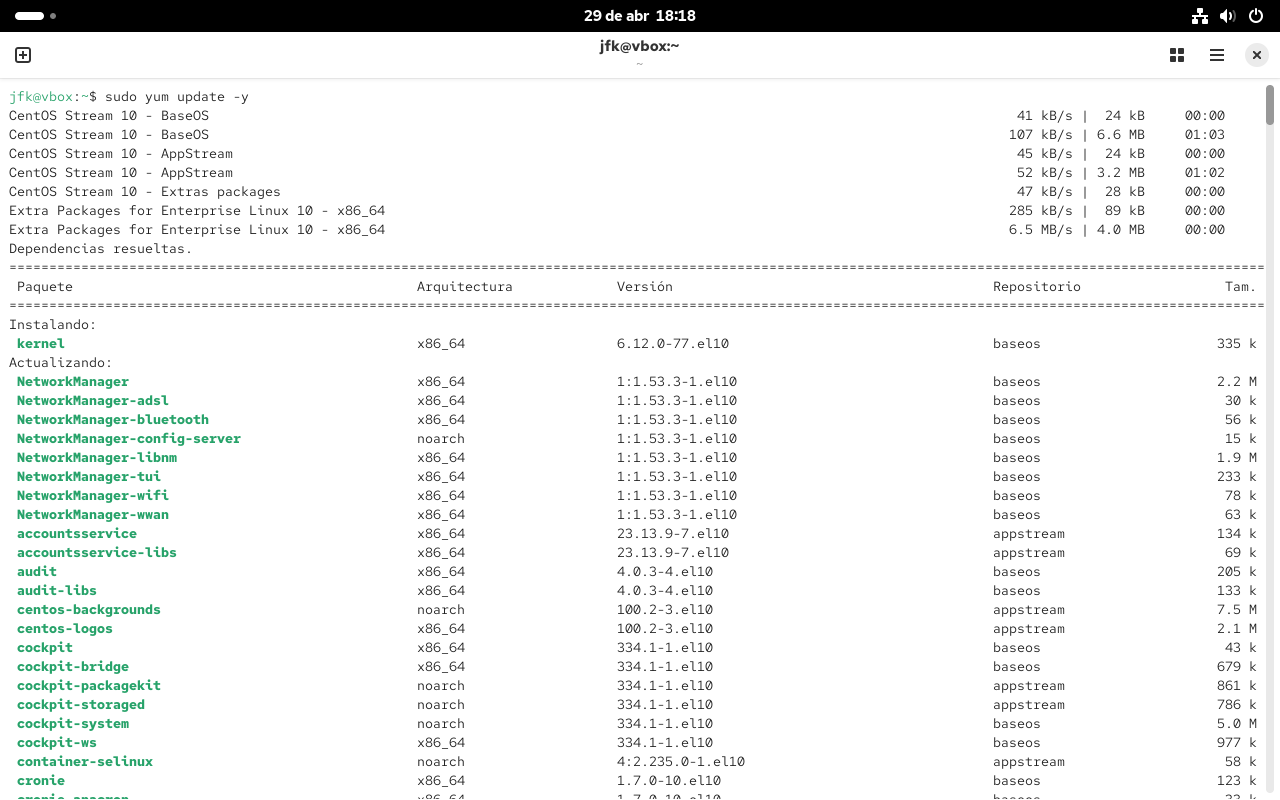
\includegraphics[width=1\linewidth]{actualizacion del sistema.png}
    \caption{Actualización del sistema}
    \label{fig:anexo1}
\end{figure}

\begin{figure}[H]
    \centering
    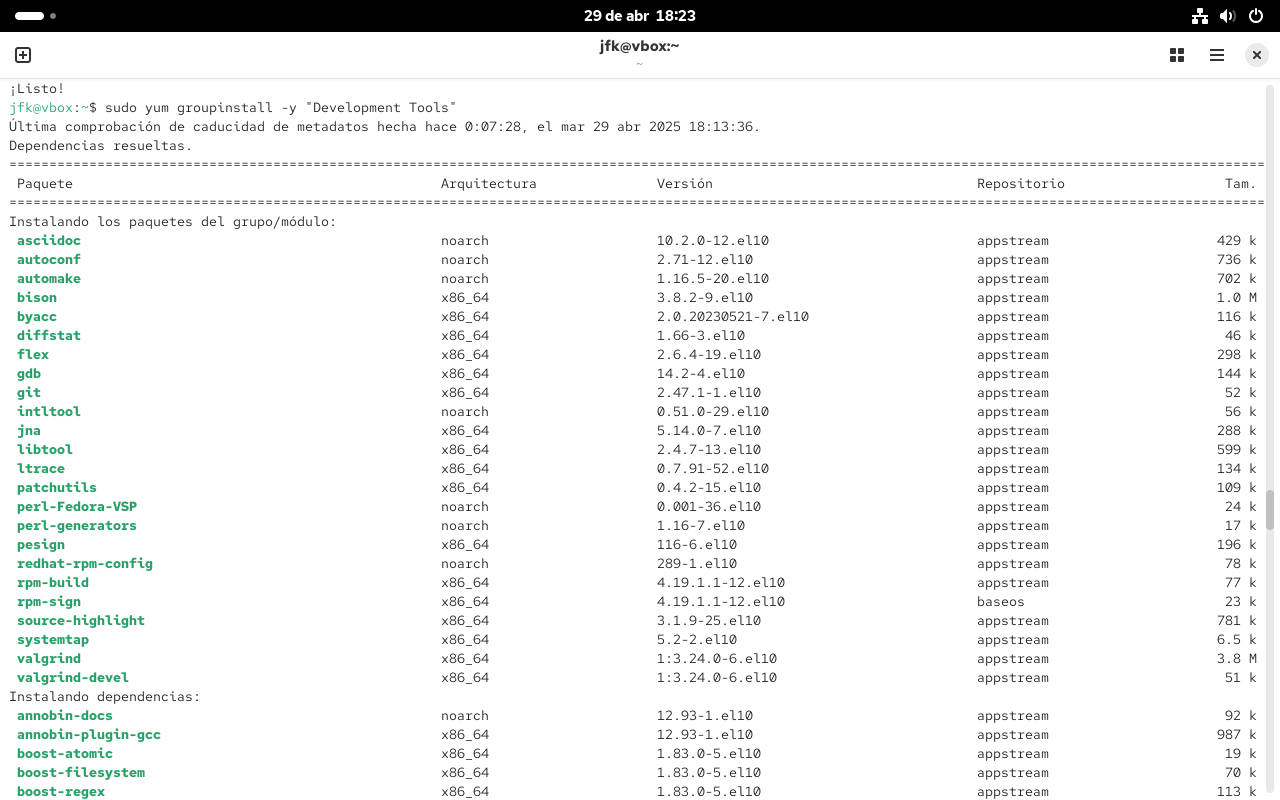
\includegraphics[width=1\linewidth]{instalacion paquetes de desarrollo necesarios para compilar OpenMPI 1.png}
    \caption{Instalación paquetes de desarrollo necesarios para compilar OpenMPI 1}
    \label{fig:anexo2}
\end{figure}

\begin{figure}[H]
    \centering
    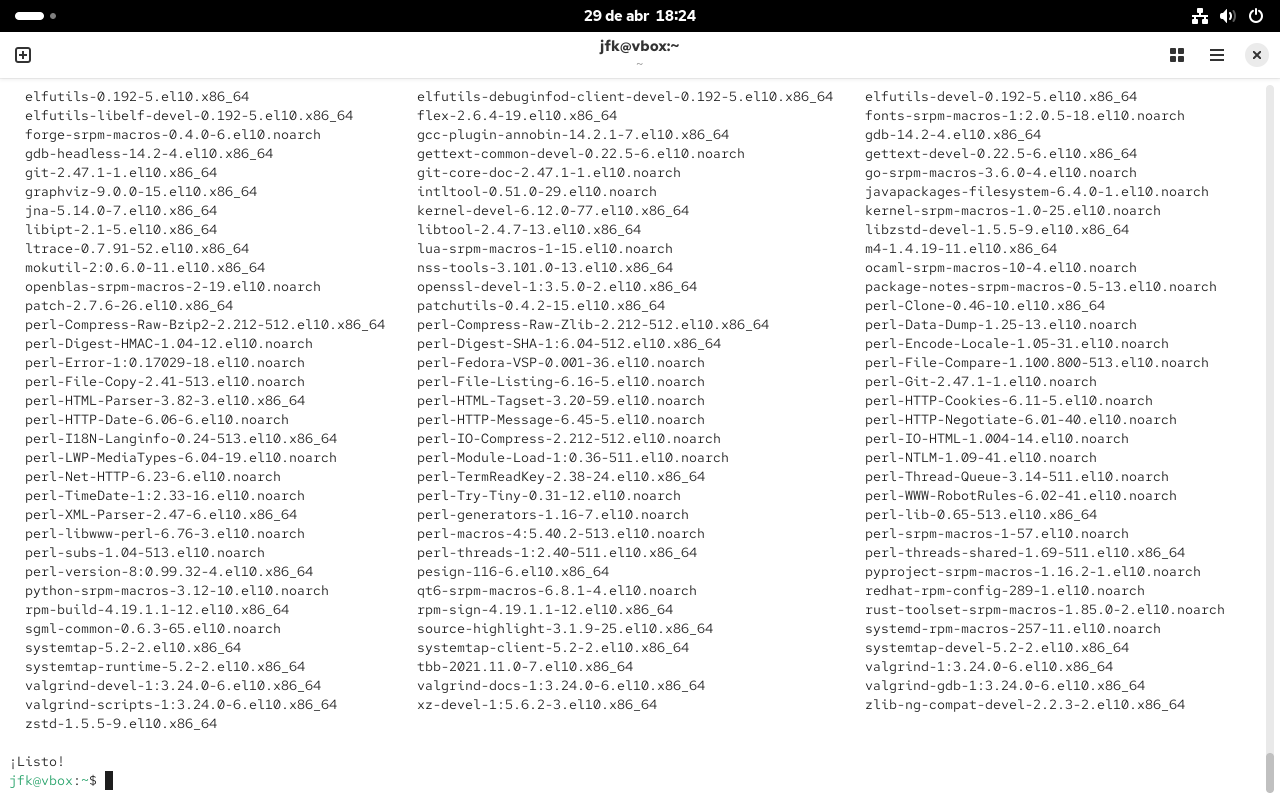
\includegraphics[width=1\linewidth]{instalacion paquetes de desarrollo necesarios para OpenMPI 2.png}
    \caption{Instalación paquetes de desarrollo necesarios para compilar OpenMPI 2}
    \label{fig:anexo3}
\end{figure}

\begin{figure}[H]
    \centering
    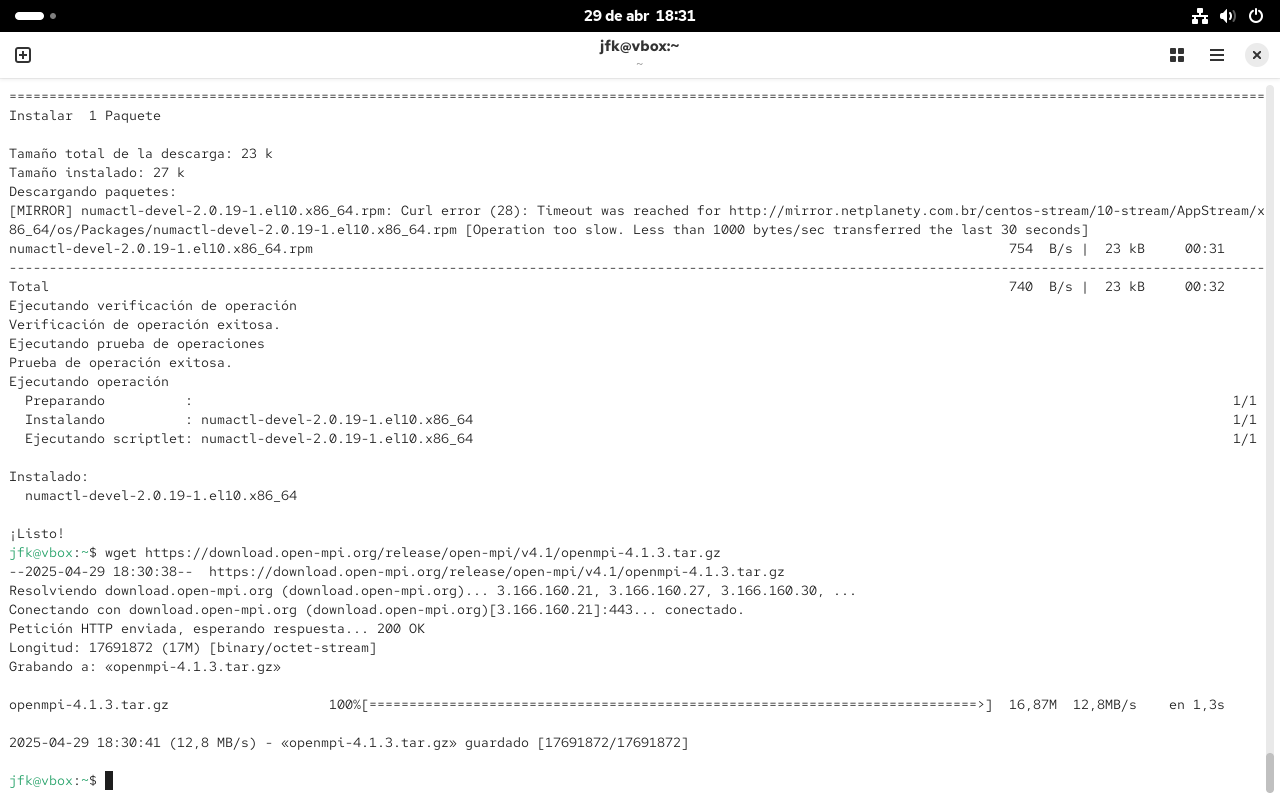
\includegraphics[width=1\linewidth]{descarga la ultima version de OpenMPI desde sitio oficial 4.1.3.png}
    \caption{Descarga de la ultima versión de OpenMPI}
    \label{fig:anexo4}
\end{figure}

\begin{figure}[H]
    \centering
    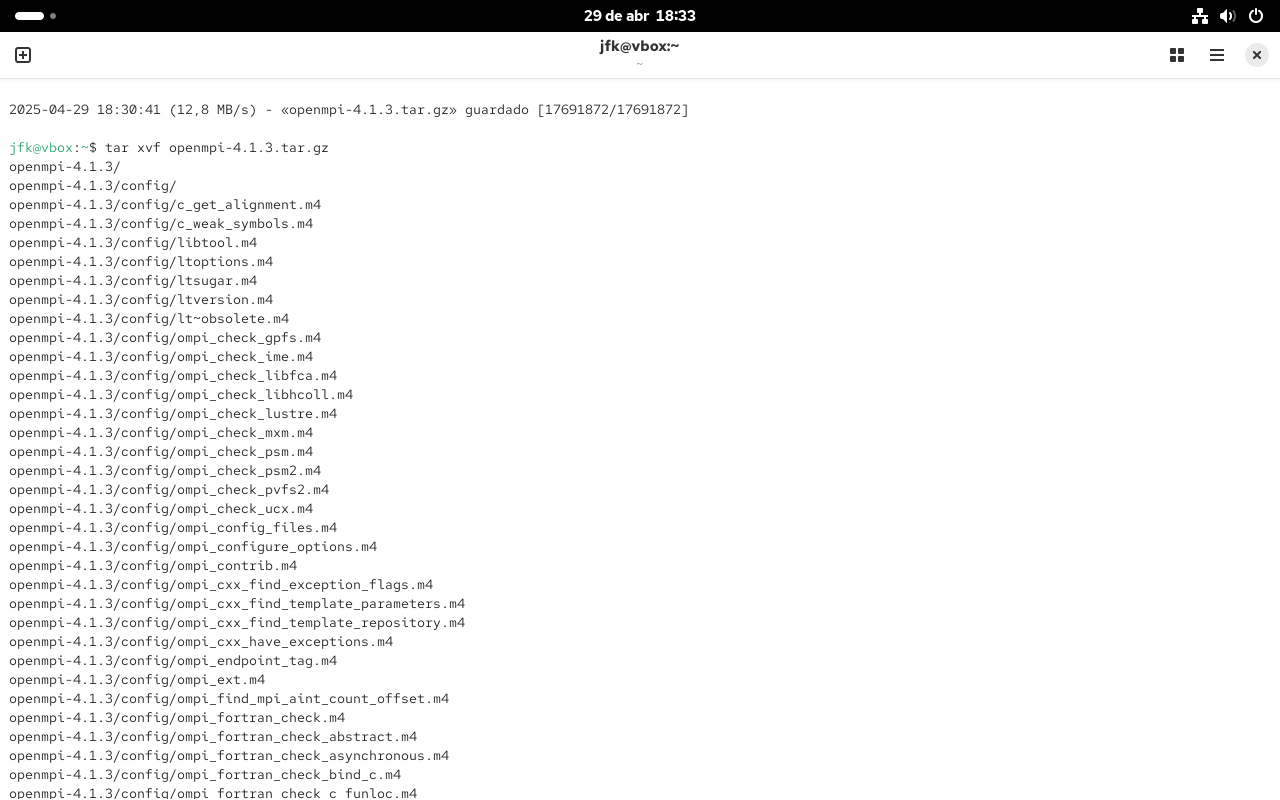
\includegraphics[width=1\linewidth]{extraer archivo comprimido.png}
    \caption{Extraer archivo comprimido de OpenMPI}
    \label{fig:anexo5}
\end{figure}

\begin{figure}[H]
    \centering
    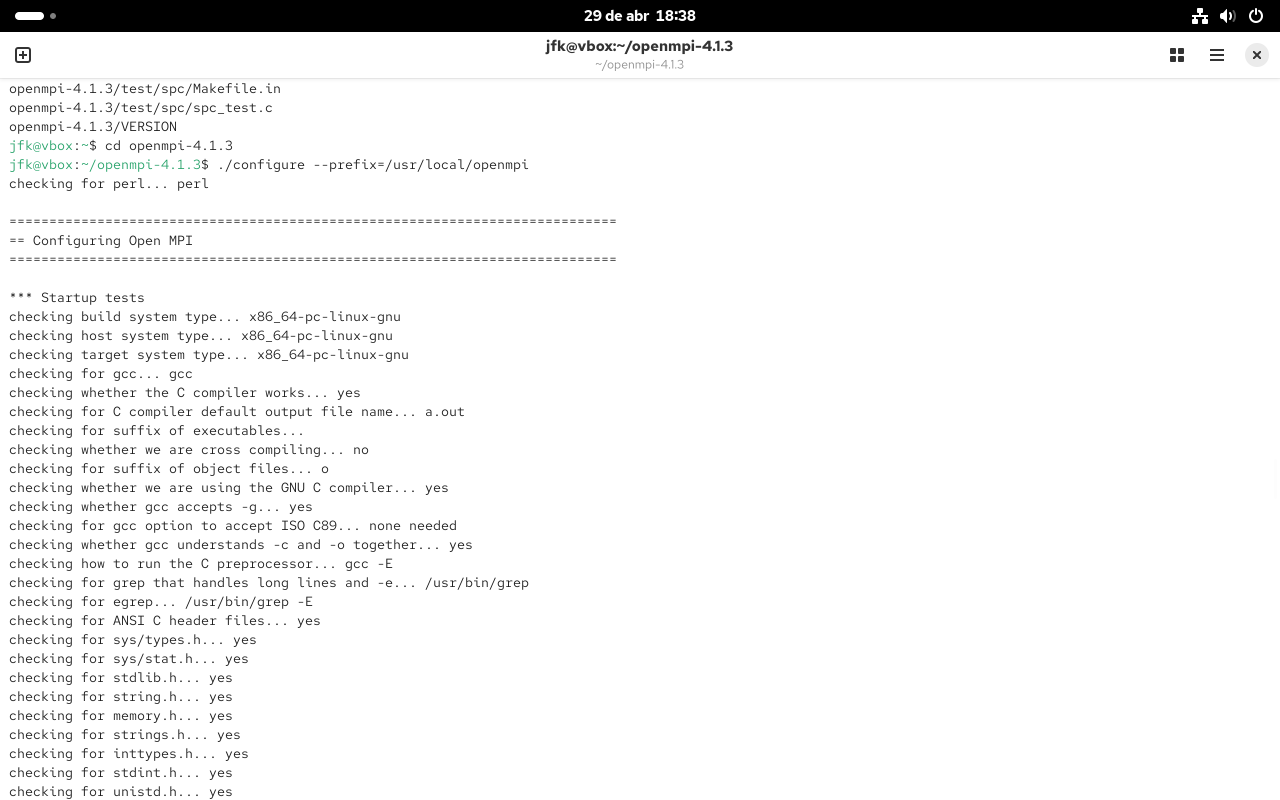
\includegraphics[width=1\linewidth]{configurar y compilar OpenMPI.png}
    \caption{Configurar y compilar OpenMPI 1}
    \label{fig:anexo6}
\end{figure}

\begin{figure}[H]
    \centering
    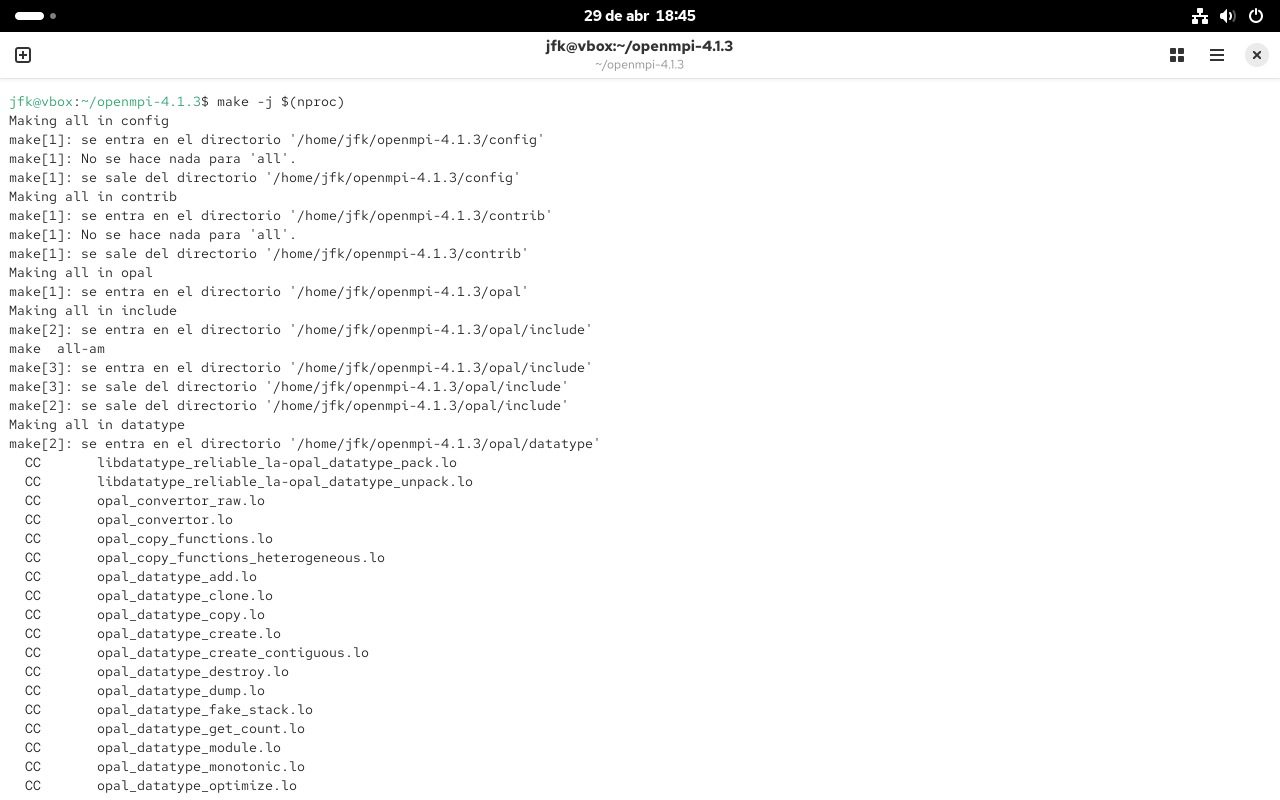
\includegraphics[width=1\linewidth]{configurar y compilar OpenMPI 2.png}
    \caption{Configurar y compilar OpenMPI 2}
    \label{fig:anexo7}
\end{figure}

\begin{figure}[H]
    \centering
    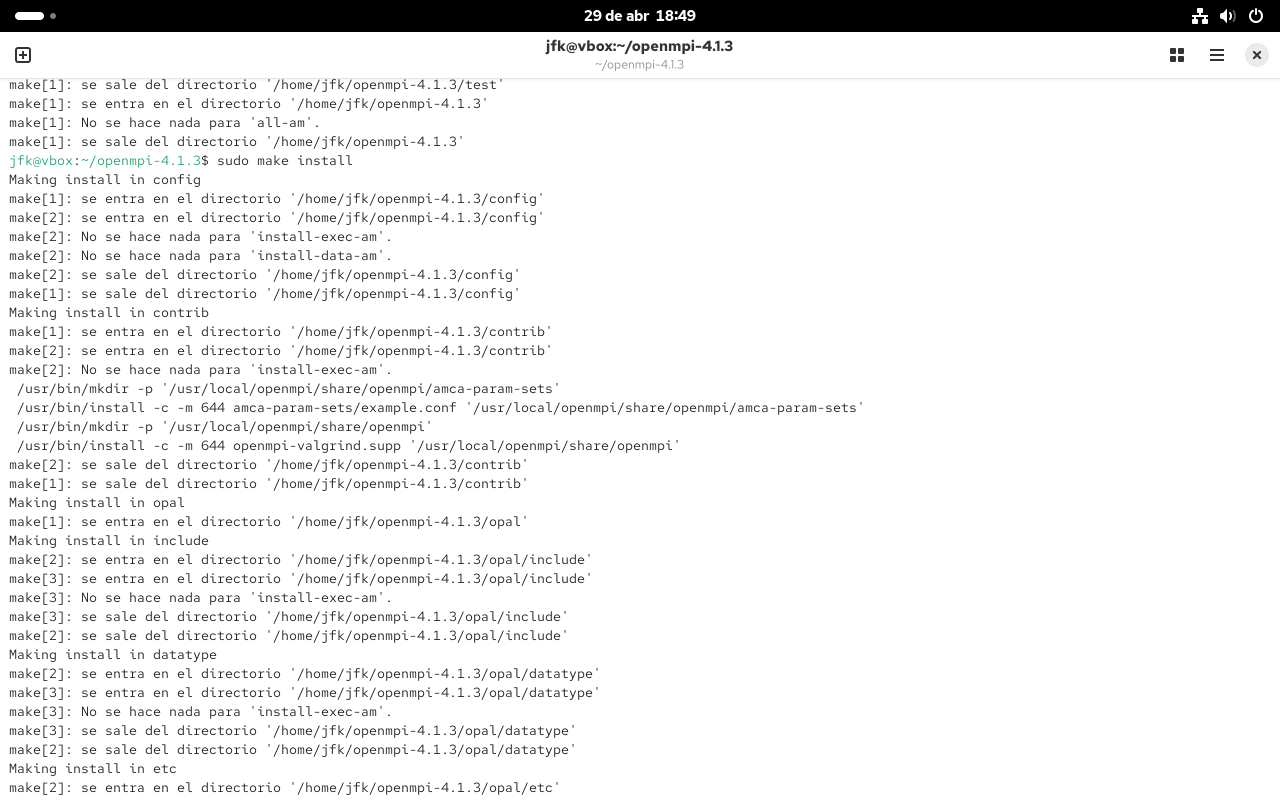
\includegraphics[width=1\linewidth]{instalacion OpenMPI en sistema.png}
    \caption{Instalación de OpenMPI en el sistema}
    \label{fig:anexo8}
\end{figure}

\begin{figure}[H]
    \centering
    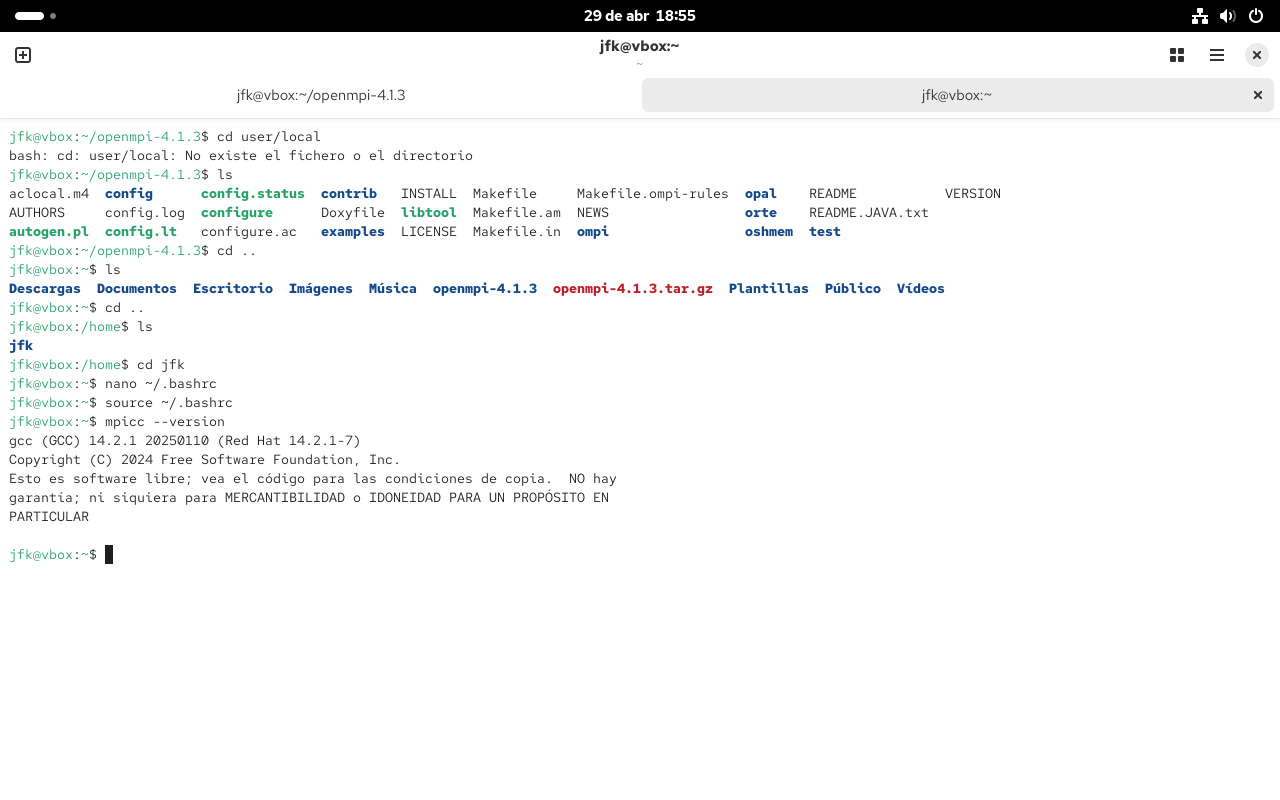
\includegraphics[width=1\linewidth]{configurar variables de entorno.png}
    \caption{Configurar variables de entorno y verificación de instalación OpenMPI}
    \label{fig:anexo9}
\end{figure}

\begin{figure}[H]
    \centering
    \includegraphics[width=1\linewidth]{compilacion y ejecucion codigo FINAL.png}
    \caption{Compilación y ejecución del código (ejemplo C++/MPI, no Java)}
    \label{fig:anexo10}
\end{figure}

\begin{figure}[H]
    \centering
    \includegraphics[width=1\linewidth]{visualizacion matrices con paralelizacion 9x9_10x10.png}
    \caption{Visualización de matrices 9x9 y 10x10 (ejemplo C++/MPI, no Java)}
    \label{fig:anexo11}
\end{figure}

\begin{figure}[H]
    \centering
    \includegraphics[width=1\linewidth]{visualizacion codigo backtracking paralelo con MPI 1.png}
    \caption{Visualización código en editor nano (backtracking paralelo C++/MPI)}
    \label{fig:anexo12}
\end{figure}

\begin{figure}[H]
    \centering
    \includegraphics[width=1\linewidth]{visualizacion codigo main backtracking MPI 2.png}
    \caption{Visualización código en editor nano (main C++/MPI)}
    \label{fig:anexo13}
\end{figure}

\end{document} 